

\begin{figure}
  \begin{subfigure}[t]{\textwidth}
    \centering
    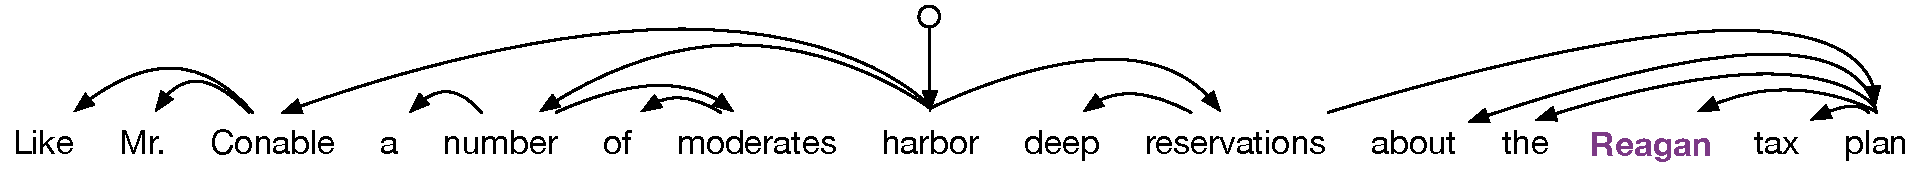
\includegraphics[width=.65\textwidth]{figures/clause_deletion/clause_deletion_one.pdf}
    \caption[]{An untyped dependency parse tree %\cite{Nivre2016UniversalDV} 
    of an input sentence mentioning $Q$=``Reagan.''}\label{f:clause_deletion_1}
  \end{subfigure}\hfill
  \begin{subfigure}[t]{\textwidth}
    \centering
    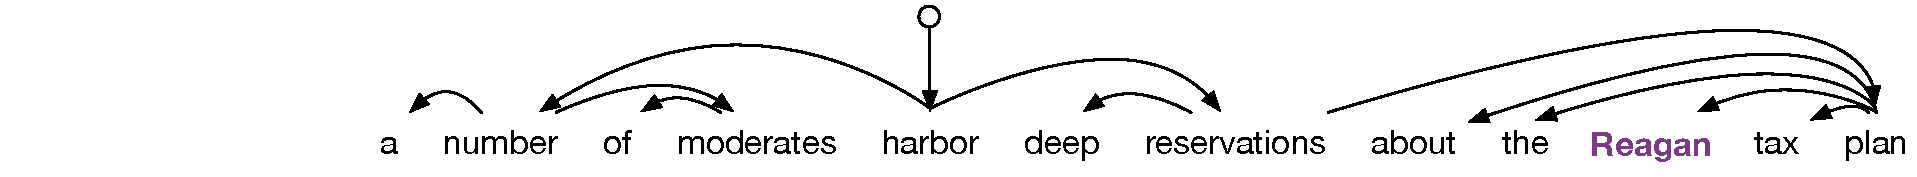
\includegraphics[width=.65\textwidth]{figures/clause_deletion/clause_deletion_two.pdf}
    \caption[]{To simplify the sentence, \ours~ first removes the clause (subtree) ``Like Mr. Conable.''}\label{f:clause_deletion_2}
  \end{subfigure}
   \begin{subfigure}[t]{\textwidth}
    \centering
    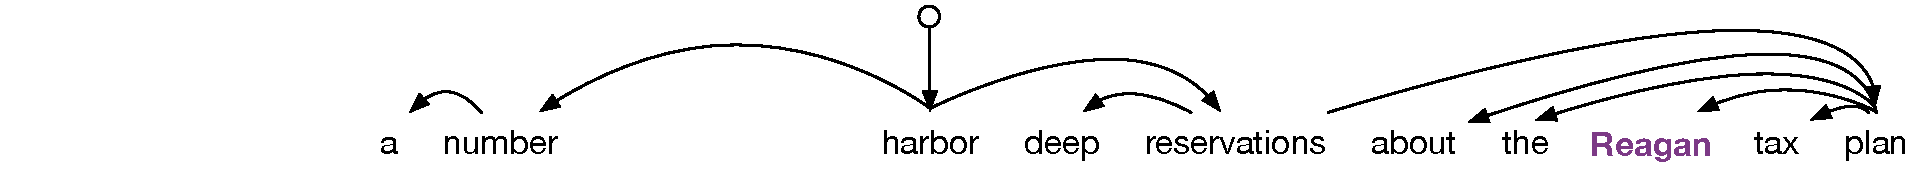
\includegraphics[width=.65\textwidth]{figures/clause_deletion/clause_deletion_three.pdf}
    \caption[]{In this step, \ours~removes another clause that does not contain $Q$.\vspace{.25 cm}}\label{f:clause_deletion_3}
  \end{subfigure}
  \caption[Sentence simplification via query-focused clause deletion]{Sentence simplification via query-focused clause deletion \cite{Handler2019Query,Handler2019HumanAJ}. \ours~removes two subtrees from a dependency parse across two steps to simplify the input sentence (\ref{f:clause_deletion_1}) into the output sentence (\ref{f:clause_deletion_3}).}\label{f:clause_deletion}
\end{figure}
